%% progress-report-8-SubmapVisualization+ROSPackage tex file.
%% Completed By Yuyang Rong(rongyy@shanghaitech.edu.cn) and
%% Jianxiong Cai(caijx@shanghaitech.edu.cn)
%%
%% To edit this file, please use indentions with tab size of 2.
%%

%% File name unchanged. This is just a temp file.

\documentclass[conference,compsoc]{IEEEtran}
\usepackage{cite}
\usepackage{listings}
\usepackage{blindtext}
\usepackage{enumitem}
% for coding highlight
\usepackage{graphicx}
\usepackage[colorlinks=true,urlcolor=blue]{hyperref}
\usepackage{amsmath, amsthm, amssymb}
\usepackage{subfloat}
\usepackage{ulem}
\usepackage{indentfirst}
\newcommand{\subparagraph}{}
\begin{document}
\title{
	Deep Learning Course Proposal \\
	Passenger Screening Algorithm Challenge \\
}


% author names and affiliations
% use a multiple column layout for up to three different
% affiliations
\author{
	\IEEEauthorblockN{Yuyang Rong}
	\IEEEauthorblockA{
		School of Information Science and Technology \\
		ShanghaiTech University \\
		Student ID: 69850764 \\
	}
\and
	\IEEEauthorblockN{Peng Ding}
	\IEEEauthorblockA{
		School of Information Science and Technology \\
		ShanghaiTech University \\
		Student ID: 79406120 \\
	}
}

\maketitle

\begin{abstract}
	The safety issue has always been a major concern since the day that aviation was civilianized. Dectecting whether passengers are carrying any prohibited items is one of the key steps before passenger board the plane. Conventionally, passengers are required to be screened and physically examined by TSA staffs. Such procedure takes time and effort to operate, without guaranteeing the accuracy of checking. Whereas complaints call upon the invasion of personal privacy. With all these being considered, people rarely consider the traditional security check as a satisfactory experience. We propose a computer vision approach, utilizing deep learning method by examining 17 critical positions of human gestures, to facilitate with the detection of prohibited items.
\end{abstract}
\section{Introduction}
	\par
	This is a Kaggle challenges proposed by the Department of Homeland Security, USA, asking for algorithms that can improve the accuracy of protential threats detection based on screening in airport. Traditional screening plus manual check approach is time consuming and facing ever increasing difficulty as the potential threats are also developing into even advanced level. With the help of up-to-date advanced learning algorithm, tackling this problem not only intrigue us to do more study but also sparking high potential value to the safety of millions of aviation passengers around the globe.
	\par
	In our work, we will be focusing on the examine of 17 key regions of a human body, as listed below:
	\begin{figure}[h]
		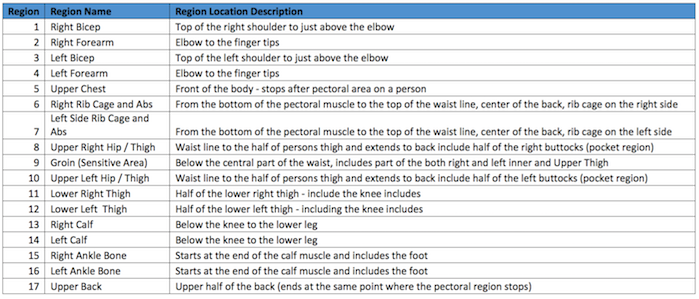
\includegraphics[scale=0.35]{Pic/body_zones.png}
		\caption{17 regions of a human body}
	\end{figure}
\section{Data}
	We will use data provided by Kaggle, to be more precise, by the Department of Homeland Security, USA. All the data are packed in the following four formats:
	\begin{itemize}
		\item{*.ahi} Calibrated object raw data file.
		\item{*.aps} Projected image angle sequence file.
		\item{*.a3d} Combined image 3D file.
		\item{*.a3daps} Combined image angle sequence file.
	\end{itemize}
\section{Approach \& Related Work}
	\par
	Ever since \cite{hinton2006fast} proposed BP, Deep learning has achieved a lot in terms of CV, speech recognition, NLP, etc.
	Years after that, more efficient and robust algorithms like SGD\cite{bottou2010large, lecun2012efficient}, BatchNorm\cite{ioffe2015batch}, Dropout\cite{hinton2012improving, srivastava2014dropout} have also been proposed. It is especially interesting to do projects on Computer Vision when ConvNet\cite{krizhevsky2012imagenet} has shown great potential in terms of accuracy.
	\par
	In our project, we will adopt ConvNet to do the recognition of potential threating objects. Also, well-respected approaches, such as the dropout mentioned above, will be tried and tested.
\section{Experiments}
	We will conduct experiments on validation set to tune our hyper-parameters. We will compare the loss function wrt. the prediction and the ground truth. The loss function is defined as follow: \\
	If there are $N$ images, there will be $17N$,
	$$ L = -\frac{1}{N}\sum_{i=1}^N{y_i\log(\hat{y}_i) + (1-y_i)log(1-\hat{y}_i)}$$
	Graphical illustration such as plotting loss vs. each parameters will be carefully selected for the result demonstration.
\section{Evaluation}
	Final evaluation will not be limited to validation set, but we will evaluate our system based on the rating algorithm proposed by Kaggle. We shall see how our kernal works after the submission.


\bibliographystyle{IEEEtran}
%% De-comment this line if you have any reference.
%% And don't forget to change .bib file.
\bibliography{proposal}
\end{document}
